\documentclass[a4paper,twocolumn]{article}
\usepackage{ucs}
\usepackage[T2A]{fontenc}
\usepackage[utf8]{inputenc}
\usepackage[english,bulgarian]{babel}
\usepackage{graphicx}

\begin{document}

\title{Code (E-Lab) Веб систем за автоматско компајлирање, извршување и
тестирање едноставни програми}

\author{М-р Томче Делев}

\maketitle

\begin{abstract}

Code е веб систем кој се развива и користи на Факултетот за информатички науки и
компјутерско инженерство и кој овозможува компајлирање, извршување и тестирање
на едноставни програми од почетнички курсеви за програмирање. Целта е да се
поедностави, подобри и подобро организира процесот на решавање задачи кои
вклучуваат програмирање. Системот е целосно веб базиран и севкупната работа на
студентите се одвива во текстуален уредувач за код во веб прелистувачот, додека
компајлирањето, извршувањето и тестирањето се одвива на веб сервер. Системот ги
подржува програмските јазици C, C++, Java и Python, а може лесно да се проширува
и за останати. Во овој труд се опишани дизјанот и имплементацијата, методите за
тестирање на решенијата и кратка на анализа на досегашното користење во рамките
на 3 различни курсеви. Исто така се дискутираат идеи за понатамошно истражување
во областа на компјутерската едукација и новите можности кои ги нудат ваквите
системи како еден вид на автоматизирани тутори.

\end{abstract}

\section{Вовед}

Програмирањето е една од основните практични вештини која се изучува на многу
предмети во курикулумите од компјутерските науки. Совладувањето на оваа вештина
им ги зголемува шансите на студентите во наоѓањето на добра работа и креирањето
на успешна кариера. Вистинска мотивација за стекнување на оваа вештина најчесто
доаѓа од можноста за добро вработување, но и од постојаниот раст на пазарот за
програмери. Сето ова ги прави факултетите од компјутерските науки многу
популарни меѓу средношколците. Крајниот резултат се голем број на студенти во
воведните курсеви, со бројки кои надминуваат стотици студенти.

Меѓутоа, програмирањето е вештина која тешко се совладува. Според некои
истражувања, потребни се и до десет години, за вистински да се научи да се
програмира. Колку и да изгледа едноставно, изучувањето на програмирање носи
големи предизвици и потребна е добра организација со вистинските алатки. Во
воведните курсеви за програмирање изучувањето најчесто значи решавање на многу
едноставни алгоритамски примери.

\section{Лабораториски вежби}

На Факултетот за информатички науки и компјутерско инженерство, практичната
работа студентите ја изведуваат преку дел од наставата наречен лабораториски
вежби. За практично да се изведуваат овие вежби потребно е студентите да се
поделат во помали групи и да се подготват повеќе компјутерски лаборатории во кои
ќе се изведуваат овие вежби. Секоја група студенти е надгледувана и оценувана од
демонстратор или асистент.

Меѓутоа иако ваквата организација за практично решавање задачи е сосема добра за
помал број студенти, со создавањето на почетни курсеви кои ги слушаат и преку
500 студенти се покажува како доста сложена за организирање и изведување. Кога
стотици студенти секоја недела работат на одредена вежба со неколку задачи, се
создаваат илјадници обиди за решенија во форма на изворен код кој треба да се
прегледаат и оценат.

Во сегашната околина студентите работат на работни станици (персонални
компјутери) во одреден текстуален уредувач или интегрирана околина за развој
(IDE) за програмскиот јазик кој го изучуваат. Тие ги зачувуваат, компајлираат и
извршуваат решенијата на нивните локални машини. Откако ќе завршат со вежбата,
не постојат никакви записи од нивната работа и не постои можност инструкторите
да ги прегледуваат или оценуваат решенијата по завршувањето на времето за
вежбата. Секоја група од студенти има временски ограничен термин од 90 до 120
минути, а самите инструктори имаат најмногу до 30 минути да ги прегледаат,
тестираат и оценат сите студенти во групата за која се одговорни. Вообичаено
една група брои 20 студенти, со што се создаваат преку педесет решенија кои
треба да се оценат. Во ваква поставеност, речиси е невозможно за инструкторите
квалитетно да ја прегледаат работата на студентите, а и во случаите кога е тоа
возможно, сепак претставува многу мачен и досаден процес.

\section{Идејата за Code}

Во основа најголем дел од задачите со програмирање во воведните курсеви се
алгоритамски по природа. Ова значи дека е возможно да се создаде платформа за
креирање задачи, тест случаи и систем кој автоматски ќе ги прегледува и оценува
решенијата. Речиси сите алгоритамски задачи може да се дизајнираат така што ќе
вчитуваат некакви податоци од стандарден влез во одреден формат и структура, да
се примени алгоритмот врз нив, а на крај да се прочита излезот од алгоритмот и
да отпечати на стандарден излез во одреден формат. Со ваков вид на проблеми може
да ја земеме извршната програма, да и ги внесеме влезните податоци и потоа го
споредиме излезот од оваа програма со очекуваниот тест излез. Со оваа споредба
може лесно да дојдеме до информација за точноста на решението. Овој процес, кој
на широко се користи во многу системи за натпревари за програмирање, треба да ја
потенцира важноста во програмирањето да се има решение кои работи точно, наместо
само да се пишува код кој понекогаш и воопшто не се компајлира.

Code е систем кој е развиен со неколку цели. Првата и основна цел беше да се
подобри организацијата и имплементацијата на практичните вежби со програмирање,
но и други значајни цели се да се мотивираат студентите преку постојаните
повратни информации за точноста на нивните решенија кои ги добиваат од системот.
Со овој систем сакаме да ја поместиме улогата на инструкторите од учители и
оценувачи кон мотиватори, нешто што се има покажано дека постигнува многу
подобри резултати во учењето програмирање.

\section{Слични системи}

Системи кои автоматски оценуваат задачи од програмирање се дизајнираат и
користат повеќе од четириесет години. Во (Douce, at al)  авторите прават преглед
и оценка на неколку значајни системи за автоматско тест-базирано оценување на
задачи од програмирање. Овие системи категоризирани се според староста во три
генерации. Првата генерација ја сочинуваат првичните системи за оценување кои
потекнуваат од времето кога се програмирало со картички и евалуацијата се
правела со извршување на програмите и рачно проверка на излезот. Некои од овие
првични системи имале специјално дизајнирани програми да го споредуваат излезот
од извршувањето со некој предефиниран излез. Втората генерација, или системи за
оценување базирани на алатки, се развивале со помош на постоечки алатки кои ги
нуди оперативниот систем или околината за програмирање. Еден значаен пример на
овие системи е системот BOSS кој потекнува од Универзитетот Варвик во
Обединетото Кралство кој, во неговите последни верзии, се разви во систем за
управување со оценките. Друг пример е проектот Scheme-Robo, кој има свој
графички кориснички интерфејс и компонента за анимација на алгоритмите. Третата
генерација на системи за оценување се карактеризираат со користење на последните
достигнувања во веб технологиите и адаптираат напредни пристапи за тестирање.
Претходно споменатиот систем BOSS еволуираше во систем од оваа генерација. Други
примери од оваа последна трета генерација се CourseMarker, развиен на
Универзитетот во Нотингем и RoboProf развиен во Универзитетот во Даблин.


\begin{figure*}[ht]
\centering
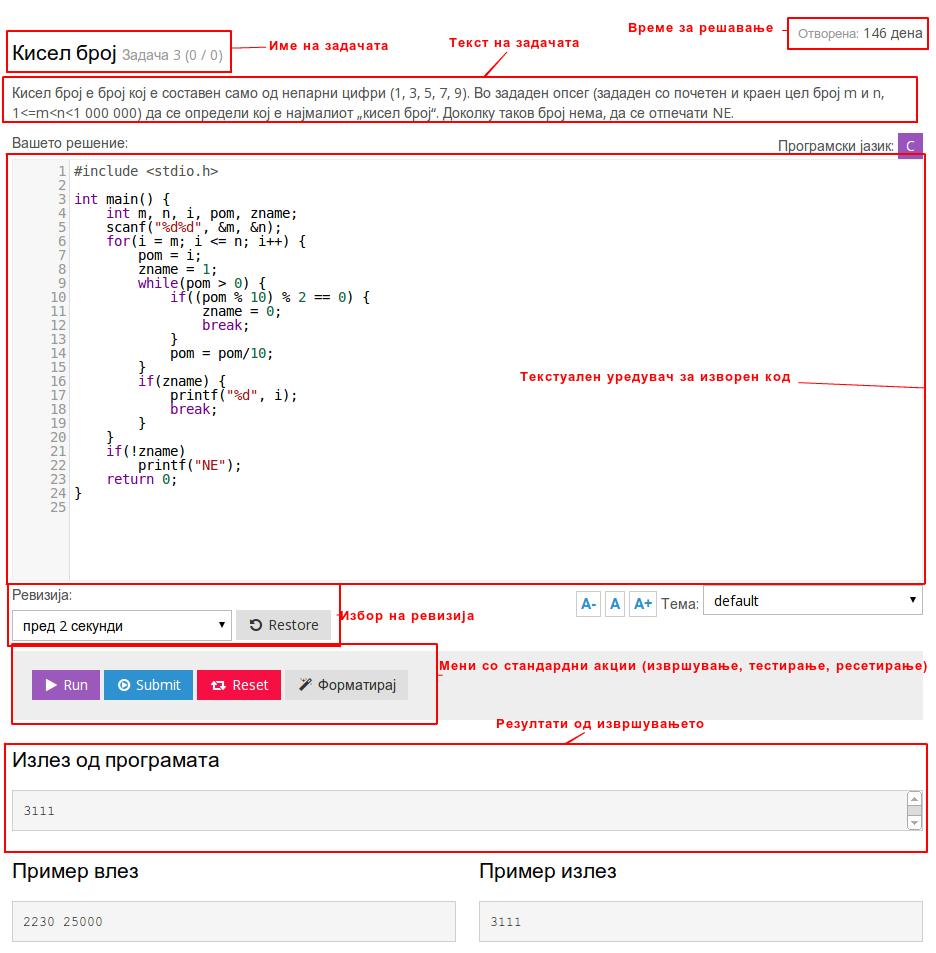
\includegraphics[width=.99\textwidth]{images/integrated_code_view}
\caption{The student screen trying to solve a problem.}
\label{fig:student_screen}
\end{figure*}


\section{Дизајн и имплементација}

Code е развиен со идејата дека треба да се изгради со користење на најновите веб
технологии и најмодерни алатки кои се имаат докажано дека функционираат преку
повеќегодишното нивно користење. Резултатот е можна четврта генерација систем,
каде што ги интегрираме последните технологии да креираме модерен, лесно
проширлив, скалабилен и најважно систем кој е едноставен за користење. Ова се
обидуваме да го постигнеме со искористување на повеќегодишното искуство на
авторот со веб технологиите, но и искуството во работата и надгледувањето
студенти кои решаваат задачи од програмирање во воведните курсеви.

\subsection{Корисници и автентикација}

Постојат четири видови на корисници: администратори, наставници, инструктори и
студенти. Сите се најавуваат и автентицираат преку централниот систем за
автентикација на ФИНКИ (CAS), кој е заеднички за сите сервиси на факултетот.
Системот дозволува пристап само на автентицирани корисници. Ове еден од начините
на кој се избегнуваат сите малициозни намери или обиди за плагијаризам, затоа
што идентитет на секој корисник е познат.

\subsection{Интегриран поглед на задачата и решението}

При обидот да се реши некоја задача студентите најголем дел од времето го трошат
во три фази. Во првата фаза го читаат текстот на задачата и се обидуваат да ја
разберат. Во втората фаза времето се посветува обидувајќи да се реши задачата,
притоа референцирајќи се на дел од содржината од курсот која е поврзана со
задачата. Резултатот од оваа фаза треба да биде пишување на програмскиот код во
одреден програмски јазик, што претставува нивното решение на задачата. Во
третата и финална фаза се одвива тестирањето на решението, односно детално
анализирајќи го излезот од системот се добива информација за точноста на
решението.

Со оглед на оваа опсервација, системот е дизајниран така што на еден екран
студентите може да работат и ги комплетираат сите фази во решавањето на
задачата. Како што може да се види на слика 1, на еден единствен поглед се наоѓа
текстот на задачата, веб-базиран текстуален уредувач за код во кој се пишува
решението и панел со акции како извршување и тестирање. Преку овие акции се
извршува решението и се добива резултат за точноста. Со овој дизајн се
имплементира пристап кој се базира на вредностите и практиките кои се дел од
начинот на учење преку извршување, заедно со постојана повратна информација за
резултатот од извршувањето.

OVDE SLIKA

\subsection{Дизајн на задачи}

Централниот ентитет во вежбите со програмирање се задачите. Секоја задача се
дизајнира во две фази. Во првата фаза се дефинира името, текстот на задачата,
тежината и потенцијален почетен код. Овие информации ја дефинираат само основата
на задачата, така што во втората фаза потребно е да се напише референтно решение
со чија помош со дадени влезни тест примери ќе се генерираат излези за сите тест
случаи. За секоја задача може да се додаде и дополнителна помош. На Слика 2 е
прикажан погледот за креирање нова задача.

\subsection{Автоматско оценување}

Ограничените ресурси во време и очигледните потешкотии со кои се соочуваат
инструкторите кои се обидуваат да ги оценат сите решенија на студентите за
одредена задача му даваат најголем приоритет на автоматското тестирање и
оценување. Системот може автоматски да оценува задачи од програмирање кои се
дизајнирани така што може да се тестираат со методот на тестирање како црна
кутија. За секоја задача авторот создава референтно решение, со кое што се
генерираат неколку тест случаи. Секој тест случај се состои од влез и излез во
текстуален формат. Кога системот тестира едно решение, ако успешно се
компајлира, извршната верзија се извршува со вчитување на влезните податоци од
тест случајот и ако е точно решението излезот од ова извршување треба да биде
идентичен со излезот од тест случајот. Една задача мора да им барем еден тест
случај кој се зема како пример за подобро да се разбере самата задача, а може да
има вкупно до десет тест случаи. Од сите тест случаи одреден процент може да
бидат скриени, односно да не може да се види влезот и очекуваниот излез со што
се оневозможува решение прилагодено само за тест случаите. При самото извршување
на програмата, ако истата не заврши во времетраење дефинирано со самата задача
(зададено три секунди), тогаш извршувањето се извршува со соодветна порака дека
во времето кое е дефинирано програмата не завршила. На Слика 3 е прикажан
погледот за креирање тест случаи за една задача.

\section{Архитектура}

\begin{figure}[ht]  
\centering
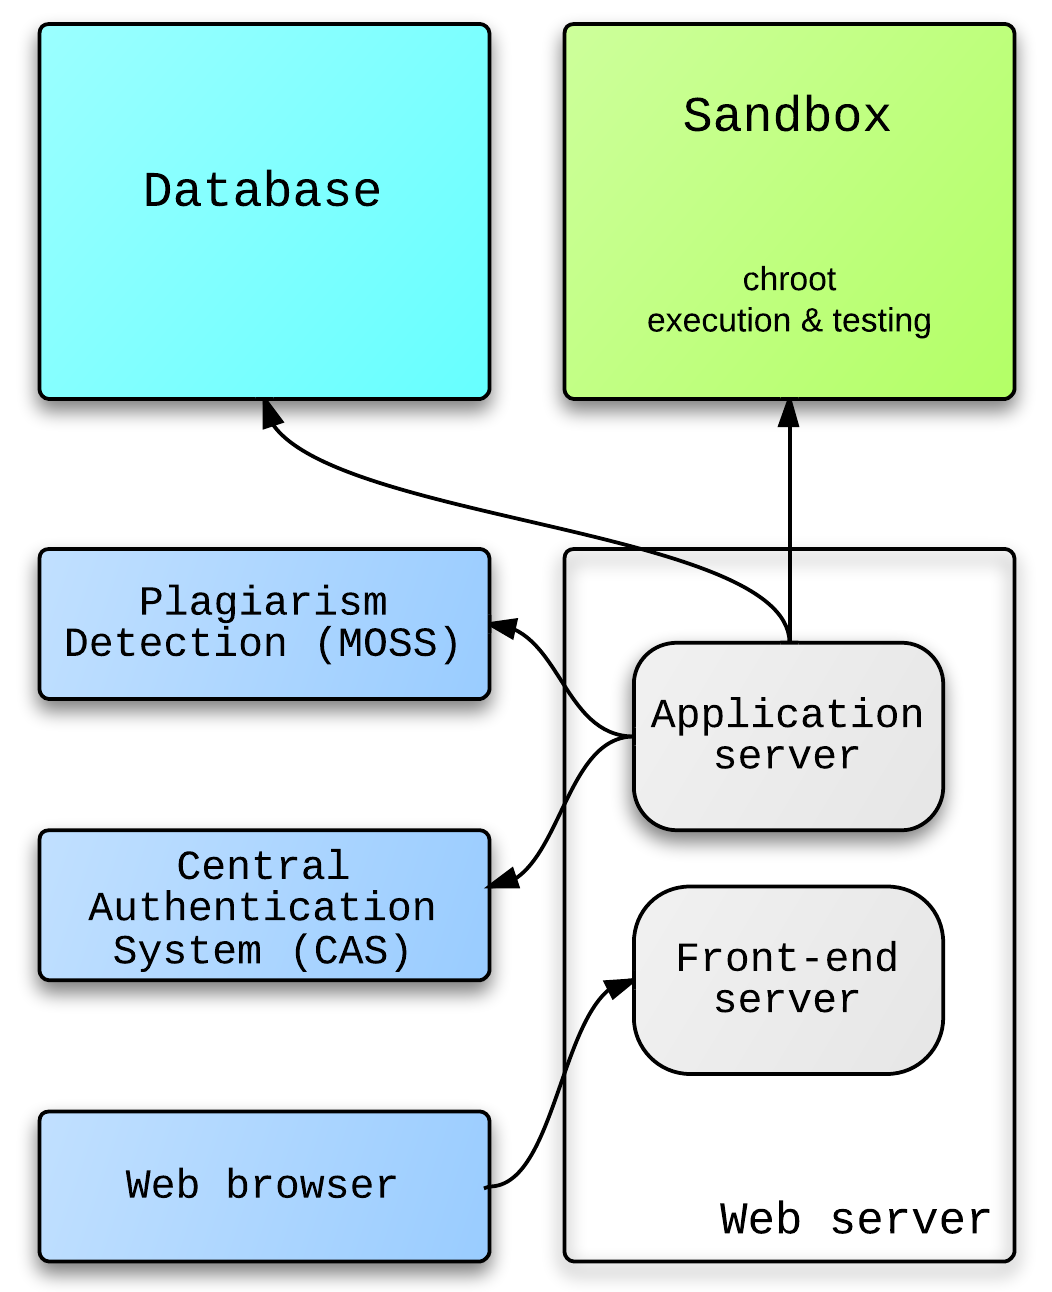
\includegraphics[width=.45\textwidth]{images/architecture}
\caption{The E-Lab architecture.}
\label{fig:architecture}
\end{figure}

На Слика 4 е прикажан преглед на архитектурата на системот, преку прикажување на
основните компоненти од кои е составен. Системот е дизајниран со модуларна
слоевите архитектура, во која основни компоненти се базата на податоци, веб
серверот и веб прелистувачот. Надворешни компоненти во архитектурата се
централниот систем за автентикација (CAS) и системот за откривање на плагијати.
Многу значаен е и заштитениот дел за извршување (sandbox) во кој се тестираат
сите решенија на задачите.

\subsection{Клиент-сервер}

Системот е форма на стандардна клиент-сервер веб архитектура. Оваа архитектура
овозможува клиентите, кои се стандардни веб прелистувачи достапни на сите
платформи, да се извршуваат на буквално сите компјутери во компјутерските
лаборатории. Ова значително ги намалува трошоците и времето за подготовка и
одржување на лабораториите, затоа што нема потреба од инсталација на специфичен
софтвер како компајлери, интегрирани околини за развој, текстуални уредувачи и
слично.

Веб серверот е составен од два посебни сервери. Пристапниот сервер е многу брз
веб сервер кој служи како прокси и распоредувач на товарот пред пристапот до
апликацискиот сервер. Апликацискиот сервер е Java сервер кој користи скалабилна
RESTfull базирана архитектура. Веб апликацијата на серверот е стандардна MVC
(Model View Controller) архитектура.

\subsection{Дијаграм на базата на податоци}

baza na podatoci

\subsection{Асинхроно извршување}

Во нашата архитектура, како и во повеќето веб базирани архитектури, серверот на
веб апликацијата треба да извршува кратки барања. За таа цел користи ограничено
множество на нитки за обработување на барањата кои се во редот за чекање на HTTP
врските. За да се остварат оптимални резултати, множеството со нитки треба да
биде што е можно помало. Оптималната вредност е бројот на процесори + 1.

Ова значи дека ако барањето трае многу долго, како што е на пример барање за
извршување на програма која не може да заврши во одреденото време за извршување
(3 секунди), ќе го блокира множеството со нитки и со тоа значително ќе влијае на
перформансите на апликацијата. Секако, може да додадеме повеќе нитки во
множеството, но ова само ќе троши системски ресурси и секако е ограничено.

Во примерот кога корисниците испраќаат за тестирање решенија кои треба да се
тестираат на 3 тест случаи и секој од овие решенија го троши целото време
дозволено за извршување (3 секунди), тогаш барањето ќе трае 9 секунди (3 тест
случаи по 3 секунди). Кога 10 корисници симултано ќе се обидат да ги испратат
своите решенија, серверот има потреба од барем 10 нитки за извршување. Овој број
е реален, но ако сакаме да имаме скалабилен систем кој подржува стотици или
повеќе корисници, потребен е друг пристап.

Во овие случаи, веб рамката која се користи ни овозможува привремено да го
паузираме извршувањето на барањето. HTTP барањето ќе остане поврзано, но
извршувањето ќе биде извадено од множеството со нитки и ќе биде продолжено
подоцна. На овој начин, сите барања кои имаат операции на извршување кои траат
долго ги извршуваме на асинхрон начин. За вакво извршување се користи нешто што
се нарекува “Asynchronous job”, и додека овие “jobs” се извршуваат, HTTP
барањето е паузирано и го чека резултатот да биде готов. Кога ќе се заврши
асинхроното извршување, HTTP барањето продолжува и резултат се враќа на
корисникот.

\subsection{Заштитено извршување}

Системот овозможува студентите да пишуваат и испраќаат секаков можен програмски
код кој ќе се извршува на оддалечен сервер. Ова може да нанесе штета на серверот
на многу непосакувани начини. Малициозниот код може да чита и запишува на
серверот, може да создава бомби од процеси, алоцира огромна меморија или
едноставно да ја троши цела процесорска моќ на серверот. За да се контролира и
заштити од ваквите безбедносни проблеми, извршувањето се прави заштитена
“sandbox” околина. Во оваа околина секое извршување е со ограничено процесорско
време и меморија, како и во бројот на процеси кои може да ги креира.

\section{Откривање на плагијати}
    
 Плагијаризмот на изворен код е сериозен проблем и мора многу јасно да им се
 воочи на студентите дека системот автоматски нема да толерира каков било вид на
 плагијаризам. Кога бројот на решенија не е многу голем може рачно да се
 споредат решенијата за плагијати, но кога имаме голем број на решенија не сме
 во можност ова да го спроведеме. Системите за автоматско откривање на плагијати
 се тема на многу студии и постојат многу системи кои се достапни на интернет.
 
Во системот Code интегриран е еден овие системи со цел да се превенира и открие
секој обид за плагијаризам. Го користиме системот MOSS развиен од Alex Aiken на
UC Berkeley. Системот “Measure Of Software Similarity” овозможува објективно и
автоматски да се проверат сите решенија и да се откријат можните случаи на
плагијати и едноставно копирање. Системот работи со програмските јазици C, C++,
Java, Python и многу останати. Стратегијата на користење во нашиот систем е да
им презентираме на студентите дека нивните решенија ќе се проверуваат дали се
плагијати. Сепак некои од наједноставните решенија мора да бидат исклучени од
проверка, затоа што можноста за концептуално различни решенија е значително
мала.

\section{Користени технологии}

Во разивањето на системот се користени следните технологи:
 PlayFramework, веб рамка
•   MySql, база на податоци
•   nginx, веб сервер
•   jQuery (Javascript библиотека)
•   Twitter bootstrap (CSS рамка)
•   CodeMirror, веб базиран текст уредувач за код
•   MathJax, библиотека за прикажување Latex на веб
•   Markdown, означувачки (markup) јазик
Системот е имплементиран (поставен) на виртуелен Linux сервер со Ubuntu 12.04 дистрибуција со следните технички спецификации:
•   Процесор Intel Xeon x5680 x 3.33 GHz 4vCPU
•   RAM 2 GB

\section{Податоци за користење}

\subsection{Корисници}

Системот има вкупно 1498 активни корисници од кои:
•   1350 студенти
•   36 инструктори
•   10 наставници
•   2 администратори

\subsection{Курсеви}

На системот моментно до сега се активирани и активни четири курсеви од зимскиот семестар:
•   Концепти за развој на софтвер (I година задолжителен, 692 студенти)
•   Алгоритми и структури на податоци (II година задолжителен, 545 студенти)
•   Напредно програмирање (II година изборен, 75 студенти)
•   Структурирано програмирање (I година задолжителен, 80 студенти)

\subsection{Задачи и решенија}

Вкупно се креирани 437 задачи групирани во 91 група на задачи (вежби, испит и домашни работи).
Вкупно се регистрирани 177012 обиди за решавање, од кои 63253 се точни, односно
околу 35\%. Просечниот број на обиди по една задача е 442.

\subsection{Испити и колоквиуми}

Досега на системот успешно и без никакви проблеми се одржани 7 колоквиуми и 3 испити.

\section{Conclusion} 

Со развојот и воведувањето на системот Code се обидуваме да решиме повеќе
организациски аспекти од изведувањето на вежби и испити од многу курсеви на
ФИНКИ кои вклучуваат програмирање. Се обидуваме да го поедноставиме и подобриме
процесот на создавање, уредување и управување со голем број задачи од
програмирање. Системот е фокусиран на студентите и нивната индивидуална работа,
додека улогата на инструкторите е да ги мотивираат и им помагаат во процесот на
создавањето на решенијата.

Имплементацијата на централна и надежна база на податоци со сите задачи,
решенија и активности во системот носи огромни придобивки во целиот процес на
настава и учење. Оваа база ги содржи сите решенија, сите обиди со некои од
најзначајните информации како на пример времето потребно да се реши одредена
задача. За сите решенија се води и историја на претходни верзии, со што не само
што им се овозможува на студентите да се враќаат на претходна верзија, туку и во
себе содржат многу значајни информации за начинот на кои студентите учат и ги
решаваат задачите. Исто така се чуваат податоци и за грешките кои ги прават
студентите, со што може да се дојде до многу значајни информации кои се најчести
грешки, а тоа секако може да помогне во подобрување на квалитетот на наставата.
Од сите овие податоци, се извлекуваат и информации од кои се креира конечната
оценка на студентот, врз база на неговите решенија.

Со овој систем, не се обидуваме да ги решиме сите организациски или едукациски
проблеми или пак целосно да го исклучиме човечкиот фактор. Code е развиен за да
помогне во секојдневното соочување со овие проблеми и со цел да се создаде
модерна околина која ќе ги мотивира студентите да работат повеќе програмирање.

\bibliographystyle{ieeetr}

\bibliography{code}

\end{document}

